\documentclass[a4paper,11pt]{article}
\usepackage{babel}
\babelprovide[import,main]{spanish}
\usepackage[utf8]{inputenc}
\usepackage[T1]{fontenc}
\usepackage[a4paper,margin=1.5cm,top=1.2cm,bottom=1.2cm]{geometry}
\usepackage{graphicx}
\usepackage{amsmath}
\usepackage{booktabs}
\usepackage{siunitx}
\usepackage{float}
\usepackage{microtype}
\usepackage{mathpazo}
\usepackage{setspace}
\usepackage{fancyhdr}
\setstretch{1.15}

\bibliographystyle{apsrev}
\setcounter{secnumdepth}{3}
\pagestyle{fancy}
\fancyhf{}
\fancyfoot[C]{\thepage}
\renewcommand{\headrulewidth}{0pt}
\renewcommand{\footrulewidth}{0pt}
\setlength{\headheight}{14pt}
\setlength{\footskip}{14pt}

\begin{document}

\title{Coupled Oscillations: Analysis of Symmetric and Asymmetric Modes}
\author{Andrés Vinuesa Espinosa \and Jose María Martínez Herrada}
\maketitle

\begin{abstract}
This report analyzes coupled oscillations in a rigid bar connected to two springs. Frequency-response measurements were used to identify the natural, symmetric, and asymmetric modes of motion and to characterize mode splitting due to coupling. A superposition experiment was also examined to recover the slow and fast components of the composite signal. The results are consistent with the expected normal-mode behavior of a linear two-degree-of-freedom oscillator.
\end{abstract}

\section{Fundamento Teórico}
El electrón se puede ver como una onda con la hipótesis de De Broglie, que establece que toda parrtícual tiene asociad una longitud de onda dada por:
\begin{equation}
\lambda = \frac{h}{p}
\end{equation}
donde $h$ es la constante de Planck y $p$ es el momento lineal de la partícula. En el caso de un electrón, $p = mv$, donde $m$ es la masa del electrón y $v$ su velocidad.
Por tanto se tiene la siguiente igualdad:
\begin{equation}
    eV=\frac{1}{2}mv^2=\frac{p^2}{2m}
\end{equation}
De donde se obtiene la siguiente expresión para la longitud de onda de De Broglie:
\begin{equation}
    \lambda = \frac{h}{\sqrt{2meV}}
\end{equation}
Donde e es la carga del electrón y V es el voltaje aplicado. Supondremos despreciables las correciones relativistas.

Según la ley de Bragg, el haz de electrones al comportarse como una onda se difracta al incidr sobre una muestra
de grafito policristalino depositada sobre una red de cobre.
\begin{equation}
    n\lambda = 2d\sin\theta
\end{equation}
En el grafito policristalino, los planos están orientados aleatoriamente, provocando que el haz de electrones
se difracte en forma de cono, provocando anillos de interferencia.
Por la geometría del dispositivo experimental, se tiene la siguiente relación entre el radio de los anillos y el ángulo de difracción:
\begin{equation}
    sin(2\theta) = \frac{r}{R}
\end{equation}
Usaremos que para ángulos pequeños, que más adelante se comprobará que
son los únicos que podemos ver en la pantalla flourescente obtenemos que:
\begin{equation}
    r=\frac{2Rn\lambda}{d}
\end{equation}
Donde $R$ es la distancia efectiva del dispositivo, que tomamos como
\SI{65}{mm} según las especificaciones del fabricante.

\section{Metodología}
\subsection{Instrumentación}
El experimento consiste en su totalidad en medir con un calibre los radios de los anillos de difracción que se forman en la pantalla fluorescente.
Este proceso se llevó acabo con un calibre, el cual cuenta con el inconveniente de no poder curvarse para medir la esfera. 
Sin embargo, hemos considerado que en las distancias que vamos a tratar, al ser ángulos muy pequeños, la diferencia entre el arco de circunferencia
y su proyección horizontal es despreciable. Por tanto, podemos medir el radio de los anillos con el calibre y considerarlo como el radio de la circunferencia.

Para controlar el momento de los electrones, se utiliza un generador de alto
voltaje. Según la ecuación de De Broglie, el radio de los anillos varía de
forma inversa con la raíz cuadrada del potencial aplicado.
Se puede concluir entonces, que el número de los anillos que en la práctica pueden ser visibles vienen dados por el voltaje que puede suministrar nuestra fuente, en nuestro caso como máximo 5kV.
Esto tiene las siguientes implicaciones:
\begin{itemize}
    \item Solo podemos ver los primeros 2 anillos de difracción.
    \item El orden de estos anillos es 1; el orden 0 se considera el haz de
    electrones que no se difracta.
\end{itemize}

La primera afirmación se justifica considerando un potencial de
\SI{4}{kV} y una distancia interplanar de \SI{213}{pm}. Al aumentar el orden
de difracción, aumenta proporcionalmente el radio previsto; por ello, los
órdenes superiores pueden quedar fuera de la zona observable de la pantalla.
En este análisis se consideran principalmente los anillos de primer orden.
\subsection{Medida}
En este proceso se presentaron varias anomalías que se describen a continuación:
En el centro de la pantalla se presenta un punto brillante, correspondiente al haz de electrones, alrededor de este punto
se pueden ver unos anillos que no cambian de radio al variar el voltaje.
Estos anillos pueden ser causados por scattering con la propia pantalla, quemaduras infrigidas en la pantalla en otros experimentos.
Pero no los hemos considerado en el análisis puesto que no tienen correlación alguna con el voltaje R²==0

En segundo lugar, cuando se miden los dos anillos exteriores, es difícil discernir a ojo desnudo a algunos voltajes para los cuales los anillos,
no se ven de forma muy intensa, donde empieza uno y donde termian otro.
Creemos que esta es la principal fuente de error en la medida, y que puede ser responsable de las discrepancias experimentales con la teoría qeu se comentarán a continuación

Por último, se ha observado que para una distancia interplanar del grafito, se pueden tener varios órdenes de difraccion,
esto hace que observar diferentes anillos sea una tarea más díficl ya que podríamos estar teninedo órdenes de otras distancias interferiendo en la medida.


\section{Resultados}
\subsubsection{Verificacion de la hipotesis de De Broglie}
La longitud de onda de De Broglie de los electrones se ha calculado mediante
\begin{equation}
    \lambda=\frac{h}{\sqrt{2m_e eV}}.
\end{equation}
Para los potenciales aplicados, entre \SI{2480}{V} y \SI{5000}{V}, se obtienen
longitudes de onda comprendidas entre \SI{17.3}{pm} y \SI{24.6}{pm}, con un
valor medio aproximado de \SI{20.1}{pm}. Para una energía cinética media de
\SI{2.5}{keV}, la expresión anterior da \(\lambda\simeq\SI{24.6}{pm}\),
equivalente a \SI{0.246}{\angstrom}. Este orden de magnitud es consistente
con el empleado en experimentos de difracción e interferencia de electrones,
como el descrito por Tonomura et al.~\cite{tonomura1989demonstration}.

La dependencia predicha por la ecuación de De Broglie es
\begin{equation}
    r=\frac{2Rh}{d\sqrt{2m_e e}}\frac{1}{\sqrt{V}},
\end{equation}
Es decir que si representamos $r$ frente a \(1/\sqrt{V}\) se debería obtener una relación lineal, sin ordenada en el origen.
por lo que se ha representado el radio medido frente a \(1/\sqrt{V}\) y se
ha realizado un ajuste lineal. La figura~\ref{fig:radius_vs_sqrt_voltage}
muestra los datos experimentales y la recta ajustada.
\begin{figure}
    \centering
    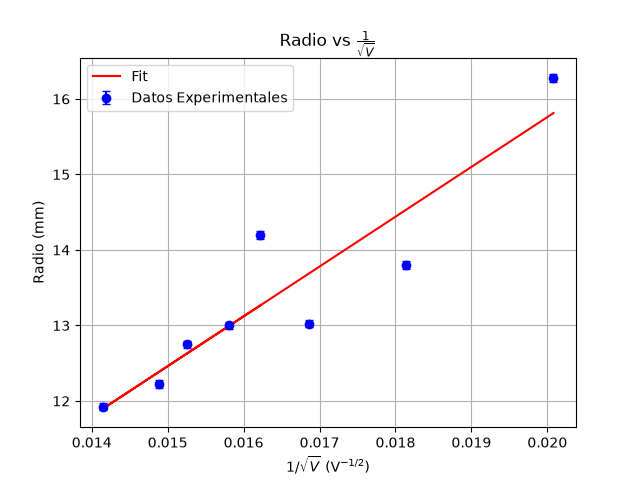
\includegraphics[width=0.5\textwidth]{radiovssqrtv.png}
    \caption{Radio del anillo de difracción en función de \(1/\sqrt{V}\).
    La linealidad de esta representación permite comprobar la dependencia
    predicha por la ley de De Broglie.}
    \label{fig:radius_vs_sqrt_voltage}
\end{figure}
El ajuste lineal proporciona los siguientes parámetros:
\begin{itemize}
    \item Pendiente: \(b=0.6598\ \si{m\sqrt{V}}\).
    \item Ordenada en el origen: \(a=0.00256\ \si{m}\).
    \item Coeficiente de Pearson: \(R^2=0.84295\).
\end{itemize}
Como el valor de \(R^2\) es cercano a 1, se puede concluir que es bastante probable que exista una relación lineal ambas variables, lo cual
apoya la validez de la hipótesis de De Broglie. 

\subsubsection{Obtencion de la segunda distancia interplanar}
También se comprobaron distintas combinaciones de orden de difracción y
distancia interplanar utilizando
\begin{equation}
    r_{\mathrm{teo}}(V;n,d)=
    \frac{2Rn}{d}\frac{h}{\sqrt{2m_e eV}}.
\end{equation}
Se consideraron los órdenes \(n=1,2,3,4\) y los valores
\(d=\SI{123}{pm}\) y \(d=\SI{213}{pm}\). Como criterio de comparación se
utilizó el error cuadrático medio entre los radios medidos y los radios
predichos.
 Si se impone que ambos
anillos proceden del mismo espaciamiento \(d=\SI{213}{pm}\) y tienen órdenes
distintos, se obtienen las dos posibilidades siguientes:
\begin{table}[H]
    \centering
    \caption{Comparación de las dos asignaciones posibles de los órdenes.}
    \begin{tabular}{lcc}
        \toprule
        Asignación & \(n\) de \texttt{radius1} & \(n\) de \texttt{radius2} \\
        \midrule
        Original & 1 & 2 \\
        Intercambiada & 2 & 1 \\
        \bottomrule
    \end{tabular}
\end{table}

La asignación original presenta un error conjunto de aproximadamente
\SI{15.7}{mm}, mientras que la asignación intercambiada presenta un error
conjunto de aproximadamente \SI{8.25}{mm}. Por tanto, si se fuerza la
hipótesis de que ambos anillos corresponden al mismo \(d\) pero a órdenes
distintos, la asignación menos desfavorable es
\[
    \texttt{radius1}\longrightarrow n=2,
    \qquad
    \texttt{radius2}\longrightarrow n=1.
\]
Sin embargo, esta hipótesis tampoco describe bien los datos. Para un mismo
valor de \(d\), la teoría predice
\[
    \frac{r_{n=2}}{r_{n=1}}=2,
\]
mientras que los datos proporcionan una razón media
\(r_{\texttt{radius1}}/r_{\texttt{radius2}}\simeq1.40\). Además, los errores
medios relativos son aproximadamente \(-45.4\,\%\) para
\texttt{radius1} como \(n=2\) y \(-21.9\,\%\) para \texttt{radius2} como
\(n=1\).

También se consideró la hipótesis alternativa en la que ambos anillos
corresponden al primer orden, pero a distancias interplanares diferentes.
Para respetar la relación inversa entre radio y distancia interplanar, se
asignó la distancia menor al radio mayor:
\[
    \texttt{radius1}\longrightarrow d_2=\SI{123}{pm},\ n=1,
    \qquad
    \texttt{radius2}\longrightarrow d_1=\SI{213}{pm},\ n=1.
\]
La comparación de ambas hipótesis se resume en la tabla~\ref{tab:hypotheses}.

\begin{table}[H]
    \centering
    \caption{Comparación entre las hipótesis de un mismo espaciamiento con
    órdenes distintos y de dos espaciamientos interplanares diferentes.}
    \label{tab:hypotheses}
    \begin{tabular}{lcc}
        \toprule
        Hipótesis & Error RMS conjunto & Error RMS relativo \\
        \midrule
        Mismo \(d_1\), \(n=2,1\) & \SI{8.25}{mm} & \SI{35.8}{\percent} \\
        \(d_2,d_1\), ambos \(n=1\) & \SI{6.00}{mm} & \SI{30.6}{\percent} \\
        \bottomrule
    \end{tabular}
\end{table}
Donde el error RMS conjunto se define como:
\begin{equation}
    \text{RMS}=\sqrt{\frac{1}{N}\sum_{i=1}^{N}(r_{\text{medido},i}-r_{\text{teorico},i})^2}
\end{equation}

Con este criterio, la hipótesis de dos distancias interplanares diferentes
describe mejor los datos: reduce el error RMS conjunto de
\SI{8.25}{mm} a \SI{6.00}{mm}. La mejora es apreciable, aunque el error
relativo sigue siendo aproximadamente del \SI{31}{\percent}, por lo que
ninguna de las dos hipótesis puede considerarse una confirmación cuantitativa
del modelo. Además, el resultado depende de la identificación de cada anillo
y de la precisión con la que se hayan medido sus radios.

\bibliography{biblio}
\end{document}